\documentclass[class=book , crop=false]{standalone}

\usepackage{import} % Required for importing other .tex docs.  (import uses everything bw Begin and End Doc)
\usepackage{float} % Required for specifying the exact location of a figure or table
\usepackage{graphicx} % Required for including images
\usepackage{wrapfig}
\usepackage[pdftex,breaklinks,colorlinks=true,linkcolor=black,citecolor=blue,urlcolor=red,linktocpage=false,pagebackref=true,filecolor=magenta]{hyperref}%http://www.tug.org/applications/hyperref/manual.html#x1-100003.6
\usepackage{cite}
\usepackage[toc,title,page]{appendix}
\usepackage{pdfpages} % enables loading a pdf into the doc
\usepackage{makeidx}
\usepackage{glossaries} % must be after hyperref
\usepackage{blindtext}
\usepackage{enumitem}
%\usepackage{caption}

%\setlist[description]{leftmargin=\parindent,labelindent=\parindent}

%\renewcommand*{\bibname}{References} % renames the bibliography

\newcommand{\HRule}{\rule{\linewidth}{0.5mm}} % Command to make the lines in the title page

\graphicspath{{img/}{GIS_ChampionSection/img/}{awardsChapter/GIS_ChampionSection/img/}{brandPart/awardsChapter/GIS_ChampionSection/img/}{img/}{pairedProgSection/img/}{methodChapter/pairedProgSection/img/}{methodPart/methodChapter/pairedProgSection/img/}{documentationSection/img/}{methodChapter/documentationSection/img/}{methodPart/methodChapter/documentationSection/img/}{docStorageOrgSection/img/}{methodChapter/docStorageOrgSection/img/}{methodPart/methodChapter/docStorageOrgSection/img/}{QGisSection/img/}{toolsChapter/QGisSection/img/}{servicePart/toolsChapter/QGisSection/img/}{ESRISection/img/}{toolChapter/ESRISection/img/}{servicePart/toolChapter/ESRISection/img/}{../../../../source/}{../../source/}{servicePart/applicationsChapter/treasurerSection/img/}}

%\setlength\parindent{0pt} % eliminates indents

\def\titlename{Jalape\~no\\ \medskip\LARGE How This Book Works}

\title{\HRule % Horizontal Line added
\\[.4cm] % space
\begin{figure}[H] % included image
\begin{center}	% centered horizontally
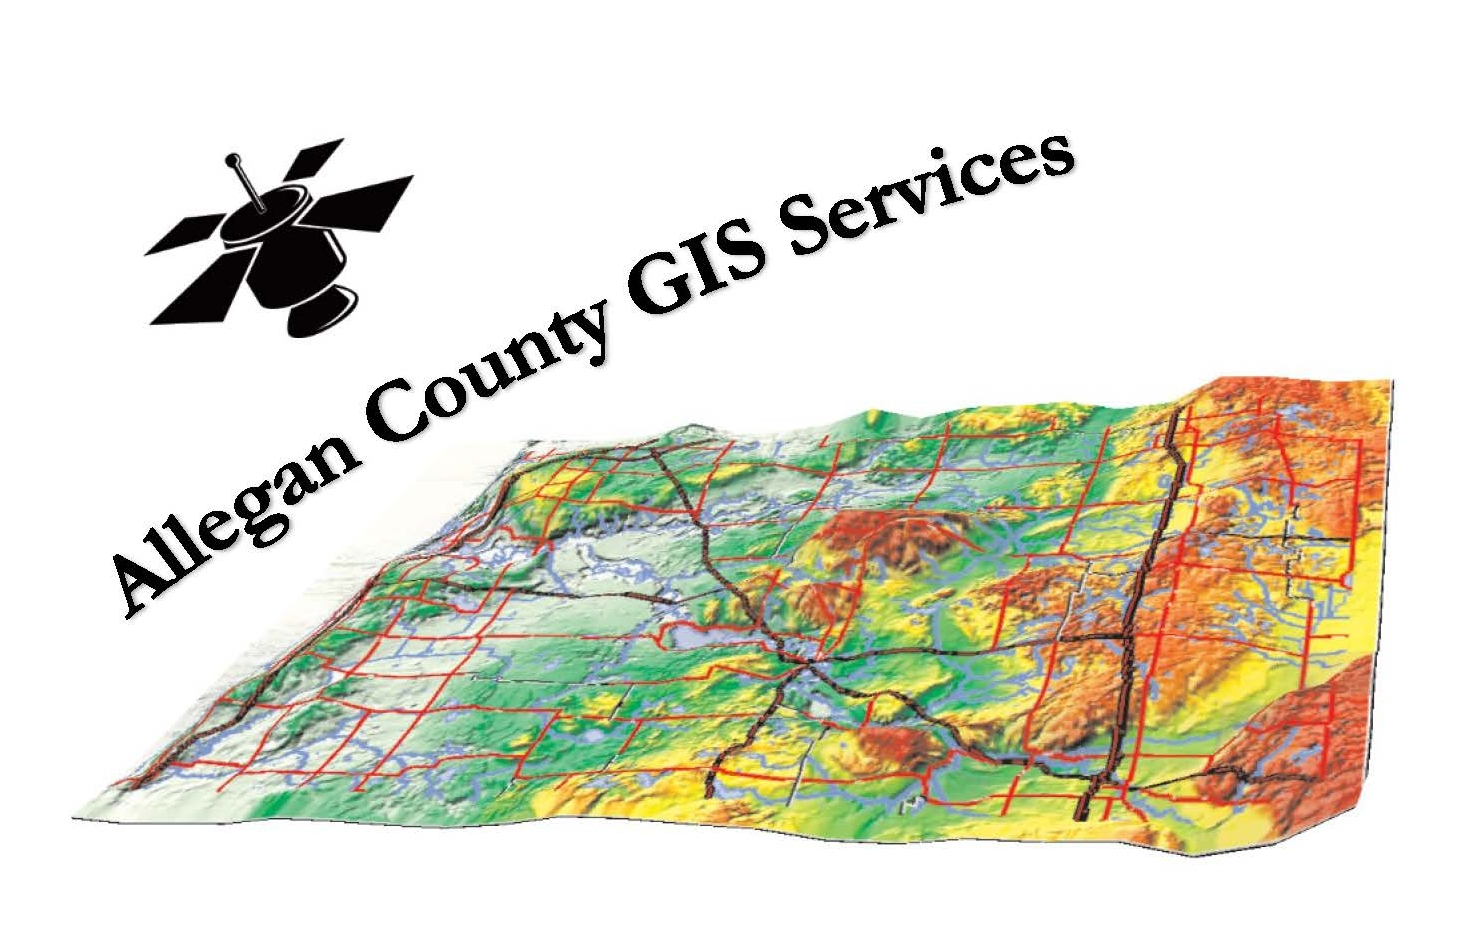
\includegraphics[scale=.45]{GIS_Logo_better.jpg}
\end{center}
\end{figure}
\Huge \bfseries \titlename \\ % Title text
\HRule \\[.4cm] % Horizontal Line added
\author{\Large Allegan County GIS \\\Large www.allegancounty.org/gis} % defines author
}  % closing brace for title

\begin{document}% Document Begins

\ifstandalone
\frontmatter % turns off chapter numbering and uses roman numerals for page numbers
\maketitle % creates title page and blank page after title page
\tableofcontents % creates TOC and blank page
\clearpage
\mainmatter % turns on chapter numbering, resets page numbering and uses arabic numerals for page numbers
\fi

\subsection{\large How \LARGE Jalape\~no \large Works}
\subsubsection{General Notes:}
\begin{itemize}
\item jalapeno folder is a git package.

\href{https://github.com/nbesteman/jalapeno}{https://github.com/nbesteman/jalapeno}

\item Project is coded with relative paths and jalapeno can be located anywhere.

\end{itemize}

\subsubsection{Project file structure:}
{\Large ...\textbackslash jalapeno\textbackslash..}\\
\begin{tabular}{p{4cm}| p{7cm} } 
folder & description \\ \hline 
documentation & resources used in Jalape\~no\\
processing & .tex douments and build folders\\
source & common image files\\
\end{tabular}
\bigskip\\
{\Large ...\textbackslash jalapeno\textbackslash documentation\textbackslash..}\\
\begin{tabular}{p{4cm} | p{7cm} } 
folder or file & description \\ \hline
moduleTemplates & .tex templates\\
packageDocs & \LaTeX{} documentation\\
references & reference and appendix resources\\
unsorted & catch all for unsorted documentation\\
BookStructureMM.mm & A mindmap of jalapeno\\
\end{tabular}
\bigskip\\
{\Large ...\textbackslash jalapeno\textbackslash processing\textbackslash..}\\
\begin{tabular}{p{4cm}| p{7cm} } 
folder or file & description \\ \hline
...Part & folders of book \textit{part}s\\
build & \LaTeX{} workspace and location of .pdf output and referenceEntries.bib* \\
commonTitle.tex & code for all title pages\\
fullCompile.sh & shell script to compile GISDocumentation.tex\\
GISDocumentation.tex & master document code\\
glossaryEntries.tex & entries that appear in glossary\\
indexEntries.tex & entries that appear in the index\\
preamble.tex & preamble code for all documents\\
\end{tabular}

\paragraph{*Note about referenceEntries.bib\\}
{\footnotesize Any reference entries built here can be cited in any .tex document in the project.}

\subsubsection{Using the glossary}
\paragraph{}
Glossary commands require a Perl interpreter.  Activeperl is a free Perl interpreter and can be downloaded from: \href{https://www.activestate.com/activeperl/downloads}{https://www.activestate.com/activeperl/downloads}
{\tiny (A typical installation adds Perl to your path)}

\paragraph{}%{Creating a glossary entry:}
\textbf{To create a glossary entry:}\\ Add an entry to glossaryEntries.tex.  Save it there but use the makeglossaries command to update the .gls file.

\paragraph{Using makeglossaries:}
In the (main document)build folder:
\begin{itemize}
\item Launch command prompt
\item enter command: \textbf{{\large makeglossaries GISDocumentation*}}
\end{itemize}
\subparagraph{*Note:} {\footnotesize This command reads the .aux file and creates the .gls file.  The .aux file is created by compiling with PDFLatex.  If there is no .aux file the command will fail.}

\subsubsection{Using the bibliography(References)}

\subsubsection{Using the Index}

\subsubsection{Using the Appendix}


\end{document}
